\chapter{Betinget sannsynlighet og uavhengighet}
\label{kap:betinget} % Opprinnelig kapittelnr: 4

Vi skal i dette kapitlet prøve å klarlegge begrepene betinget
sannsynlighet og uavhengighet, samt etablere de viktigste regnereglene
 knyttet til disse begrepene. Dette utvider vår verktøykasse for
 stokastisk modellbygging og sannsynlighetsberegning.

\section{Betingede sannsynlighetsmodeller}

Vi har et eksperiment, eller annen form for iakttakelse, med utfallsrom
\[    \Omega = \{u_1, u_2, u_3, \ldots \} \]
og sannsynligheter gitt ved
\[     P(u_1), P(u_2), P(u_3), \ldots \]

\noindent La oss tenke oss at eksperimentet er utført og at vi blir gitt
den opplysningen at en bestemt begivenhet $B$ har inntruffet. Dette
betyr at et eller annet av de gunstige utfall for $B$ har
inntruffet, vi vet bare ikke hvilket. Det er nå klart at den
opprinnelige modellen ikke nødvendigvis passer lenger. For det
første vet vi nå at en rekke utfall, nemlig alle utfall i $\bar{B}$,
ikke kan ha inntruffet. For det andre er det rimelig at
sannsynligheten for utfall som fortsatt er tenkelig bør endres.
Vi ønsker derfor å lage en modifisert modell hvor vi tar hensyn
til den tilleggsinformasjon at begivenheten $B$ har inntruffet.
  \footnote{Vi antar hele tiden at begivenheten $B$ er slik at $P(B)>0$.}

\begin{center} 
\framebox[10cm]{
\begin{minipage}{9cm}\rule{0cm}{0.5cm}
\begin{definisjon}
  Den betingede sannsynlighet $P_B(u)$ for utfallet $u$ gitt begivenheten
  $B$ er %\\
%\begin{center}
\begin{tabular}{ccll}
  $P_B(u)$&$=$&0  & for $u \in \bar{B}$ \\
        &$=$&$\frac{P(u)}{P(B)}$ & for $u \in B$ 
\end{tabular} 
%\end{center} \\[2mm]
\end{definisjon}
\end{minipage}
} 
\end{center}
Dette betyr at vi tildeler sannsynlighet null til de utfall som ikke 
lenger er aktuelle , mens vi lar det innbyrdes forhold
mellom sannsynlighetene for de utfall som fremdeles er aktuelle
være det samme som før. Det er lett å sjekke at denne
konstruksjonen oppfyller kravene A1 og A2 til en
sannsynlighetsmodell:

\[ \mbox{A1: \ \ \ \ \ \ \ }  0 \leq P_B(u) \leq 1
                             \mbox{\ \ \  for alle \ \ } u\in \Omega\]
\[ \mbox{A2:\ \ }\sum_{u\in \Omega}P_B(u)=\sum_{u\in B}\frac{P(u)}{P(B)}= 
      \frac{1}{P(B)} \sum_{u\in B}P(u)=\frac{1}{P(B)} \cdot P(B)=1\]

\noindent {\bf Merknad}. I den betingede modell gitt $B$ kunne vi bruke
$B$ som utfalls\-rom istedenfor $\Omega$. Dette kan se ut som en
forenkling, men i praksis ønsker man ofte å studere flere
betingede modeller samtidig, og da er det greitt å beholde
$\Omega$ som felles referanseramme. \\

\begin{eksempel}{Et terningkast}
Gitt modellen for et kast med en rettferdig terning:
\begin{center}
\begin{tabular}{lcccccc}
Utfall:          &    1 & 2 & 3 & 4 & 5 & 6 \\
Sannsynlighet:   & $\frac{1}{6}$& $\frac{1}{6}$& $\frac{1}{6}$&$\frac{1}{6}$&
                  $ \frac{1}{6}$& $\frac{1}{6}$
\end{tabular}
\end{center}
Etter et kast med terningen opplyses det at den ikke viste seks
øyne. Vi vet demed at begivenheten $B=\{1,2,3,4,5\}$ må ha
inntruffet. Vår intuisjon sier nå at den betingede modell gitt
$B$ bør se slik ut:
\begin{center}
\begin{tabular}{lcccccc}
Utfall:          &    1 & 2 & 3 & 4 & 5 & 6 \\
Sannsynlighet:   & $\frac{1}{5}$& $\frac{1}{5}$& $\frac{1}{5}$& $\frac{1}{5}$&
                 $ \frac{1}{5}$&$0$
\end{tabular}
\end{center}
dvs. de 5 utfall som fortsatt er aktuelle bør fortsatt ha samme
sannsynlighet. Siden $P(B)=5/6$ ser vi av definisjonen ovenfor at

\[    P_B(u)=\frac{P(u)}{P(B)}=\frac{1/6}{5/6}=\frac{1}{5}
                                    \mbox{\ \  for alle \ \  } u \in B \]

\noindent som altså stemmer med vår intuisjon. Anta isteden at
 terningen er falsk og konstruert slik at sjansen for sekser er redusert (som
medfører at sjansen for ener er øket). Anta at en brukbar modell
for et kast med denne terningen er gitt ved
\begin{eqnarray*}
 P(1)=0.19&P(2)=0.17&P(3)=0.17 \\
 P(4)=0.17&P(5)=0.17&P(6)=0.13
\end{eqnarray*}
I dette tilfelle blir $P(B)=0.87$, slik at den betingede modell blir 

%\begin{center}
\begin{tabular}{lcccccc}
Utfall:          &    1 & 2 & 3 & 4 & 5 & 6 \\
Sannsynlighet:   &$\frac{0.19}{0.87}$&$\frac{0.17}{0.87}$&$\frac{0.17}{0.87}$&
                 $\frac{0.17}{0.87}$&$\frac{0.17}{0.87}$&$0$
\end{tabular}
%\end{center}
\end{eksempel}
\\[0.2cm]
\noindent La nå $A$ være en vilkårlig begivenhet i utfallsrommet $\Omega$.
Ifølge A3 bør den betingede sannsynlighet for begivenheten $A$ gitt
$B$ være summen av de betingede sannsynligheter for de utfall som
er gunstige for $A$, dvs.

\[     P_B(A)=\sum_{u\in A}P_B(u) \]

\noindent Med denne definisjonen vil vi få de samme regneregler for
betingede sannsynligheter som for vanlige sannsynligheter (E1-E7
i kapittel 2.4). I tillegg har vi noen nye regneregler. Den første er:

\[ P_B(A)=\frac{P(A \cap B)}{P(B)} \]
{\bf Begrunnelse :} Del summen ovenfor opp i to deler, de utfall i $A$ som 
også er med i $B$, og de utfall i $A$ som også er med i $\bar{B}$.
Ifølge definisjonen av betinget sannsynlighet, er alle ledd i den siste
summen null, mens  i den første summen blir fellesfaktoren $1/P(B)$
multiplisert med en sum, som ifølge A3 er $P(A \cap B)$. Forsøk selv
å formalisere begrunnelsen.\\

Dette betyr at enhver sannsynlighet i den betingede
modell gitt $B$ kan beregnes ut fra sannsynligheter i den
opprinnelige modell.
I praksis er det vanlig å bruke en annen skrivemåte for betingede
sannsynligheter. Istedenfor $P_B(A)$ skriver man $P(A\mid B)$
hvor symbolkombinasjonen $A\mid B$ uttales ``A gitt B'', og vår
fundamentale formel lyder derfor 

\begin{center} \framebox[10cm]{\begin{minipage}{9cm}
\[ \mbox{\ \ \ E8. \ \ \ \ } P(A \mid B)=\frac{P(A \cap B)}{P(B)}  \]
 \mbox{} \end{minipage}} \end{center}


\begin{eksempel}{Korttrekning}
Et kort trekkes tilfeldig fra en kortstokk. La \\ \\
\indent     $A$ = Sort kort \\
\indent     $B$ = Honnør (ess, konge, dame eller knekt) \\ \\
\noindent Her blir
\[  P(A)=\frac{g}{m}=\frac{26}{52} \mbox{ , }
 P(B)=\frac{g}{m}=\frac{16}{52}\mbox{ , }P(A\cap B)=\frac{g}{m}=\frac{8}{52} \]
\noindent slik at
\[ P(A \mid B)=\frac{P(A \cap B)}{P(B)}=\frac{8/52}{16/52}=\frac{1}{2} \]
\noindent mens
\[ P(B \mid A)=\frac{P(A \cap B)}{P(A)}=\frac{8/52}{26/52}=\frac{4}{13} \]
\end{eksempel}

\begin{eksempel}{Poker}
Anta at alle $m=\bino{52}{5}$ mulige korthender er like sannsynlige, og la\\ \\
\indent     A = korthånden består av 5 spar \\
\indent     B = korthånden består av 5 sorte kort \\ \\
Her blir $P(B)=\bino{26}{5}/\bino{52}{5}$ og
                $P(A \cap B)=P(A)=\bino{13}{5}/\bino{52}{5}$, slik at
\[ P(A \mid B)=\frac{P(A \cap B)}{P(B)}=
         \frac{\bino{13}{5}}{\bino{26}{5}}=\frac{1\:287}{65\:780}=0.0196 \]
\end{eksempel}

\begin{eksempel}{To terningkast.}
Anta at alle $m=36$ mulige par av øyne er like sannsynlige. La \\  \\
\indent     A = Begge terninger viser 6 øyne \\
\indent     B = Minst en terning viser 6 øyne \\
\indent     C = Sum øyne er minst 10 \\  \\
Vi har $P(A)=1/36$, $P(B)=11/36$ og $P(C)=6/36$, og finner at

\[ P(A \mid B)=\frac{P(A \cap B)}{P(B)}=\frac{1/36}{11/36}=\frac{1}{11} \]
\[ P(B \mid C)=\frac{P(B \cap C)}{P(C)}=\frac{5/36}{6/36}=\frac{5}{6} \]
Det overlates til leseren å beregne flere betingede sannsynligheter :\\
 $P(B\mid A)$, $P(C\mid B)$, $P(C\mid A)$ og $P(A\mid C)$.
\end{eksempel}

\section{Regneregler for betingede sannsynligheter}

Tar vi utgangspunkt i den fundamentale formelen E8 og
multipliserer med $P(B)$ på begge sider av likhetstegnet, får vi 

\begin{center} \framebox[10cm]{\begin{minipage}{9cm}\rule{0cm}{0.5cm}
 $ \mbox{ \ \  \ E9. \ \ \ \ } P(A\cap B)=P(B)\cdot P(A\mid B) $ \\
 \rule{0cm}{0.3cm} \end{minipage}} \end{center}
Selv om denne formelen uttrykker samme saksforhold som E8,
poengterer den en annen bruksmåte: Når $P(B)$ og $P(A\mid B)$ er
kjent kan $P(A\cap B)$ beregnes. Dette vil vi dra nytte av senere
ved beregning av sannsynligheter. Dersom vi lar $A$ og $B$ bytte
rolle i E8 får vi $P(B \mid A)=P(A \cap B)/P(A)$.
Innsettes her uttrykket for $P(A\cap B)$ fra E9, får vi

\begin{center} \framebox[11cm]{\begin{minipage}{10cm}
\[ \mbox{\ \ \ E10. \ \ \ \ } P(B \mid A)=
     \frac{P(B) \cdot P(A \mid B)}{P(A)} \mbox{\bf \ \ \ \ (Bayes lov) }\]
\mbox{}  \end{minipage}} \end{center}

\noindent som er en viktig regneregel i praksis. En annen viktig regneregel
fås ved følgende betraktninger. Anta at

\[ \Omega = B_1 \cup B_2 \cup \cdots \cup B_r \]

\noindent er en disjunkt oppsplitting av den sikre begivenhet (se Figur~\ref{fig:disjunkt_oppspl}).
La $A$ være en vilkårlig begivenhet. Vi kan da skrive

\[  A=(A \cap B_1) \cup (A \cap B_2) \cup \cdots \cup (A \cap B_r) \]
Siden dette er en disjunkt union medfører E7 at

\begin{center} \framebox[12cm]{\begin{minipage}{11cm}\rule{0cm}{0.5cm}
 $ \mbox{\  E11. \ \ }
     P(A)=P(B_1)\cdot P(A\mid B_1)+P(B_2)\cdot P(A\mid B_2)+ $ 
\flushright $ \cdots +P(B_r)\cdot P(A\mid B_r) $ \\
\rule{0cm}{0.3cm} \end{minipage}} \end{center}

\begin{figure}[ht]
\centering \centering
 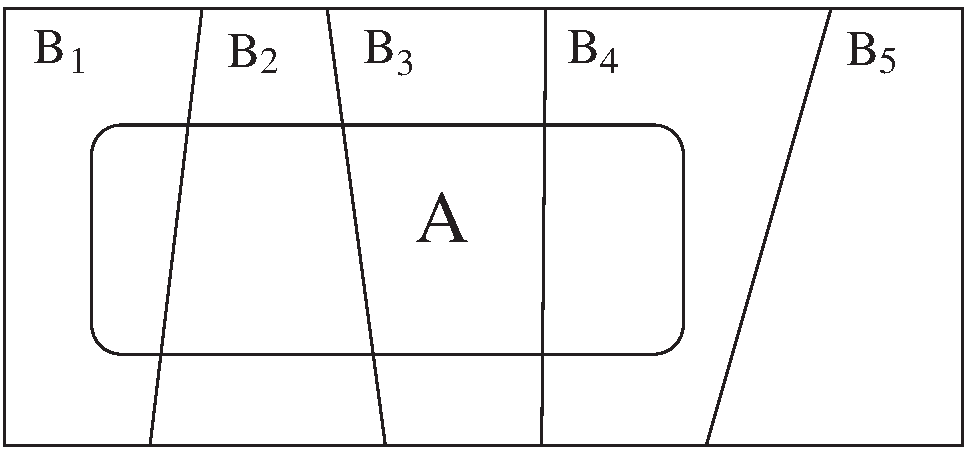
\includegraphics[scale=0.6]{figurer/fig4_1.pdf} 
 \caption{Beregning av sannsynlighet ved betinging}
	\label{fig:disjunkt_oppspl}
\end{figure}
I mange problemstillinger hvor $P(A)$ ikke lar seg beregne
direkte, er det mulig å splitte opp den sikre begivenhet på en
slik måte at sannsynlighetene på høyresiden av E11 er kjent eller
kan beregnes. Vi sier da at $P(A)$ blir beregnet ved betinging
(mhp. $B_1, B_2, \ldots B_r)$. Ved beregning av nevneren i Bayes lov
er det ofte aktuelt med betinging. Siden $\Omega =B\cup \bar{B}$ får vi
et viktig spesialtilfelle av E11:

\[  P(A)=P(B)\cdot P(A\mid B)+P(\bar{B})\cdot P(A\mid \bar{B}) \]

I mange situasjoner er det naturlig å konstruere
sannsynlighetsmodellen ved å gjøre antakelser om noen av de
betingede sannsynligheter i modellen. Når man skal løse
sannsynlighetsteoretiske problemer i praksis, hender det ofte at
man lar være å gi en fullstendig beskrivelse av
sannsynlighets\-mo\-dellen, man nøyer seg med å gjøre tilstrekkelig
mange ad hoc antakelser om modellen til at de søkte
sannsynligheter lar seg beregne. Man må da selvsagt sørge for at
de valgte antagelser ikke står i motstrid med hverandre. Nyttige
formler i denne forbindelse er nettopp E9, E10 og E11.
Sannsynligheten på venstresiden lar seg bestemme ved å gjøre
antagelser om sannsynlighetene på høyresiden.
Såkalte urnemodeller kan bidra til å klargjøre begrepene. \\

\begin{eksempel}{To urner}
Gitt to urner, den første med 4 hvite og 2 sorte kuler, den andre
med 2 hvite og 2 sorte kuler. Først velges tilfeldig en av
urnene, deretter trekkes tilfeldig en kule fra den valgte urne.
Vi ønsker å beregne sannsynligheten for at den valgte kule er
hvit. Definer begivenhetene \\ \\
\indent            $U_i=$ Urne nr. i velges, $i=1,2.$ \\
\indent            $H  =$ Hvit kule trekkes \\ \\
\noindent Tilfeldig valg av urne og tilfeldig trekning fra urnen betyr at
\[ P(U_1)=P(U_2)=\frac{1}{2} \]
\[ P(H \mid U_1)=\frac{4}{6},\;\;\;  P(H \mid U_2)=\frac{2}{4} \]

\noindent Ifølge regneformlene ovenfor får vi

\[ P(U_1 \cap H)=P(U_1) \cdot P(H \mid U_1)=
                   \frac{1}{2} \cdot \frac{4}{6}=\frac{1}{3} \]
\[ P(U_2 \cap H)=P(U_2) \cdot P(H \mid U_2)=
                   \frac{1}{2} \cdot \frac{2}{4}=\frac{1}{4} \]
slik at

\[ P(H)=P(U_1 \cap H)+P(U_2 \cap H)= \frac{1}{3} + \frac{1}{4}=\frac{7}{12}\]

\noindent mens sannsynligheten for sort kule $(S)$ blir $P(S)=5/12$. Dette
kan enten regnes ut på samme måte eller enklere ved å bruke at
$P(S)=1-P(H)$. Gitt at den uttrukne kule er hvit. Sannsynligheten
for at den kom fra urne nr. 1 blir

\[    P(U_1 \mid H)=\frac{P(U_1 \cap H)}{P(H)}=\frac{1/3}{7/12}=\frac{4}{7}\]

\noindent mens sannsynligheten for at den kom fra urne nr. 2 blir
$P(U_2\mid H)=3/7$. Dette kan enten regnes ut på samme måte eller
enklere ved å bruke at $P(U_2\mid H)=1-P(U_1\mid H)$. Det kan vi
fordi $U_1$ og $U_2$ er komplementære begivenheter (dvs. $U_2=\bar{U_1})$ og
 betingede sannsynligheter oppfyller samme
regneregler som vanlige sannsynligheter.
\end{eksempel}

\begin{eksempel}{To trekninger}
Gitt en urne med 2 hvite og 3 sorte kuler. Først trekkes
tilfeldig en kule fra urnen, deretter trekkes en ny kule
tilfeldig fra de gjenværende kuler i urnen. Definer følgende
begivenheter \\ \\
\indent     E = Hvit kule i første trekning \\
\indent     F = Hvit kule i annen trekning \\ \\
\noindent Ordet tilfeldig betyr at ved hver trekning har alle kulene i
urnen samme sannsynlighet for å bli trukket ut, dvs.
 \begin{eqnarray*} 
P(E)=\frac{2}{5}&&P(\bar{E})=\frac{3}{5} \\
P(F \mid E)=\frac{1}{4}&& P(F \mid \bar{E})=\frac{2}{4}
\end{eqnarray*}
\noindent Vi får derfor

\[ P(E \cap F)=P(E) \cdot P(F \mid E)= 
                         \frac{2}{5} \cdot \frac{1}{4}=\frac{1}{10} \]
\[ P(\bar{E} \cap F)=P(\bar{E}) \cdot P(F \mid \bar{E})= 
                         \frac{3}{5} \cdot \frac{2}{4}=\frac{3}{10} \]
og følgelig
\[ P(F)=P(E \cap F) + P(\bar{E} \cap F)= 
                         \frac{1}{10} + \frac{3}{10}=\frac{2}{5} \]
\noindent Videre blir
\[ P(E \cap \bar{F})=P(E) \cdot P(\bar{F} \mid E)= 
                         \frac{2}{5} \cdot \frac{3}{4}=\frac{3}{10} \]
\[ P(\bar{E} \cap \bar{F})=P(\bar{E}) \cdot P(\bar{F} \mid \bar{E})= 
                         \frac{3}{5} \cdot \frac{2}{4}=\frac{3}{10} \]
og følgelig
\[ P(\bar{F})=P(E \cap \bar{F}) + P(\bar{E} \cap \bar{F})= 
                         \frac{3}{10} + \frac{3}{10}=\frac{3}{5} \]
som vi kunne innsett direkte fra formelen $P(\bar{F})=1-P(F)$. En
alternativ måte å studere denne problemstillingen på er å
anta at alle $(5)_2=20$ ordnede utvalg av 2 kuler er like sannsynlige.
Det overlates til leseren å påvise at dette leder til samme
sannsynligheter. Gitt at annen trekning ga hvit kule.
Sannsynligheten for at også første trekning ga hvit kule blir

\[ P(E \mid F)=\frac{P(E \cap F)}{P(F)}=\frac{1/10}{2/5}=\frac{1}{4} \]
mens sannsynligheten for ikke hvit (sort) kule blir 3/4. Dette
kan enten regnes ut på samme måte eller ved
 $P(\bar{E} \mid F)=1-P(E \mid F)$.
\end{eksempel}


\begin{eksempel}{Tennis}
I herretennis spilles best av 5 sett, dvs. at kampen vunnet straks en av spillerne
har vunnet 3 sett. To spillere A og B som rangeres likt spiller mot hverandre. 
Hva er sannsynligheten for at A vinner kampen dersom
\begin{itemize}
\item[(a)] A har vunnet to sett og B ett
\item[(b)] A har vunnet de to første sett 
\item[(c)] A har vunnet første sett 
\end{itemize}
Vi får ved å betinge mhp. hvem som vinner neste sett
\begin{eqnarray*}
 p_a  & = & \frac{1}{2} \cdot  1  + \frac{1}{2} \cdot \frac{1}{2}  = \frac{3}{4} \\
 p_b  & = & \frac{1}{2} \cdot  1  + \frac{1}{2} \cdot p_a         = \frac{7}{8} \\ 
 p_c  & = & \frac{1}{2} \cdot p_b + \frac{1}{2} \cdot \frac{1}{2}  = \frac{11}{16} 
\end{eqnarray*}
Vi har her brukt at når begge har vunnet like mange sett,
så er sannsynligheten 1/2 for at A vinner. Vi ser at når vi regner ut
sannsynlighetene i denne rekkefølgen, kan vi bruke resultatet av
den foregåenede beregning i den neste.

Eksemplet har en viss historisk interesse som et av de første
sannsynlighetsteoretiske problemer som ble studert i det vitenskapelige
miljø, riktignok i en annen forkledning: Hva er en rettferdig deling av 
potten når et spill må avbrytes før det er ferdig?
Etter flere feilaktige løsninger på 1400-tallet, ga Pascal, Fermat og 
Huygens hver sin korrekte løsning på 1600-tallet.
Pascal og Fermat brukte kombinatoriske argumenter, mens løsningen 
ovenfor er i Huygens' ånd, selv om han ikke brukte begrepet
sannsynlighet.

Leseren kan selv forsøke å utvikle id\'{e}en videre til å løse
``best av 7-spill'', slik tilfellet er i Stanley Cup i ishockey. 
\end{eksempel}

De tre eksemplene ovenfor kan oppfattes som {\em trinnvise
eksperimenter}, dvs. at utfallet av hvert trinn definerer
betingelsene for neste trinn. I Eksempel 5 var første
trinn valg av urne, annet trinn valg av kule fra den valgte urne.
I Eksempel 6 var første trinn valg av en kule, annet trinn valg
av kule blant de gjenværende i urnen etter at den første er
trukket. I Eksempel 7 vil hvert sett være et nytt trinn.

Et trinnvis eksperiment kan beskrives ved et såkalt {\em
sannsynlighetstre}. I tilfellet med to trinn og to utfall på
hvert trinn ser et tre ut som i Figur~\ref{fig:sannsynlighetstre}. 

\begin{figure}[ht]
\centering \centering
 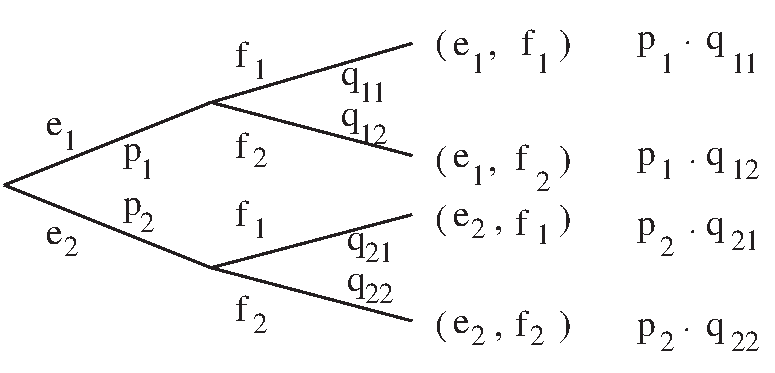
\includegraphics[scale=0.7]{figurer/fig4_2.pdf} 
 \caption{Sannsynlighetstre}
	\label{fig:sannsynlighetstre}
\end{figure}
Et sannsynlighetstre leses fra venstre mot høyre. Vi starter med
et forgreningspunkt (roten av treet) som svarer til første trinn.
Ut fra dette går grener, en for hvert mulig utfall av første
trinn (her $e_1$ og $e_2$), på hver sin gren skriver vi de
respektive sannsynligheter (her $p_1$ og $p_2$). Langs hver av
disse grener nås et nytt forgreningspunkt, som svarer til annet
trinn. Fra et slikt punkt går nye grener, en for hvert mulig
utfall av annet trinn (her $f_1$ og $f_2$), og på hver gren
skriver vi de sannsynligheter $(q_{i1}$ og $q_{i2})$ som er
aktuelle for den forgrening vi er på $(i=1$ eller $2)$, alt etter
utfallet av de foregående trinn. De ulike mulige hendelsesforløp
av eksperimentet er påført ved enden, dette svarer til de mulige
utfall av hele eksperimentet. Til hvert utfall svarer altså en
sti gjennom treet fra roten til ytterste kvist.

Vi finner sannsynligheten for hvert utfall ved å multiplisere
sammen sannsynlighetene langs den sti som svarer til dette
utfallet. Disse sannsynlighetene kan så påføres ved enden av
treet, merk at alle disse må summere seg opp til en.
Sannsynligheten for en bestemt begivenhet $A$ kan nå finnes ved å
summere de sannsynlighetene som svarer til stier som er gunstige
for begivenheten $A$. 

Et sannsynlighetstre kan være et nyttig hjelpemiddel til å gi en
oversiktlig beskrivelse av mer kompliserte
sannsynlighetsteoretiske situasjoner, dvs. trinnvise situasjoner
med mer enn to trinn og med flere (ofte varierende antall) utfall
på hvert trinn, se Eksempel 9 nedenfor Slik trebeskrivelse viser seg å
være spesielt nyttig ved analyse av sekvensielle 
beslutningsproblemer under usikkerhet (se Kapittel 16).

Vi har utelatt en formell begrunnelse for at den trinnvise konstruksjon 
ovenfor virkelig gir en sannsynlighetsmodell, og at de betingede 
sannsynligheter kan gjenfinnes fra denne. Det er ikke vanskelig, men krever
en viss formalisme, som i figuren. Leseren kan heller prøve å 
gjennomskue dette ved å lage et sannsynlighetstre, konstruere modell 
med utfall og tilhørende sannsynligheter og verifisere beregningen  
i Eksempel 5 og 6 (se Oppgave~19). 

I Kapittel 3 studerte vi bl.a. ordnede utvalg uten tilbakelegging.
Dette kan alternativt studeres som et trinn\-vis eksperiment, og det er 
kanskje slik trekningen lettest gjennomføres i praksis. Det er
lett å verifisere at tilfeldig utvelgelse på hvert trinn leder til et
tilfeldig utvalg i den forstand vi definerte det i Kapittel 3.
Nedenfor følger argumentasjonen for tilfellet med utvalg på 
to elementer, som lett kan utvides trinnvis til flere. Stoffet er
$\star$-merket og kan overspringes uten fare for å miste tråden. \\[0.2cm]
\small
$\star$ Gitt en populasjon på $N$ elementer nummerert fra $1$ til $N$.
Først trekkes tilfeldig et element, deretter trekkes tilfeldig et
nytt element fra de gjenværende $N-1$ elementer. La $e_i$ bety at
første trekning gir element nr. $i$ og $f_j$ bety at annen
trekning gir element nr. $j$. Siden hver trekning foregår
tilfeldig har vi følgende delmodeller

\begin{center}
\begin{tabular}{llcccc}
Trinn 1: & Utfall:     & $e_1$&$  e_2 $& $\ldots $ &$ e_N$ \\
         & Sannsynlighet:&$\frac{1}{N}$&$\frac{1}{N}$&$\ldots $&$\frac{1}{N}$ 
\end{tabular}
\end{center}
Dersom trinn 1 ga $e_i$ som resultat har vi følgende modell for
trinn 2:

\begin{center}
\begin{tabular}{llcccccc}
Trinn 2: & Utfall:     & $f_1$&$  f_2 $& $\ldots$ &$f_i$&$\ldots$&$ f_N$ \\
 & Sannsynlighet:&$\frac{1}{N-1}$&$\frac{1}{N-1}$&$\ldots$&$0$&$\ldots$&$\frac{1}{N-1}$ \\
\end{tabular}
\end{center}
Som utfallsrom for to-trinns eksperimentet bruker vi de ulike kombinasjonene $(e_i,f_j)$,
og to-trinnsmodellen er dermed definert ved

\begin{eqnarray*}
   P((e_i,f_j))&=&0   \mbox{   for j=i  } \\
              &=&\frac{1}{N} \cdot \frac{1}{N-1} \mbox{   for }j \ne i
\end{eqnarray*}
Siden  $\frac{1}{N} \cdot \frac{1}{N-1}=\frac{1}{(N)_2}$, ser vi at denne to-trinnsmodellen er
ekvivalent med en modell hvor vi antar at alle $(N)_2$ mulige
ordnede utvalg uten tilbakelegging er like sannsynlige. Den
eneste forskjell er at den foreliggende modell nytter et større
utfallsrom og tildeler sannsynlighet null til de utfall hvor
samme element forekommer i begge trekninger.

La oss se hvordan vi i praksis ville beregnet sannsynligheten for
begivenheten $F_j=$ annen trekning gir element nr. $j$.
La $E_i=$ første trekning gir element nr. $i$. Vi kan anta at
$P(E_i)=1/N$  og $P(F_j \mid E_i)=0$ for $j=i$ og $1/(N-1)$ for $j \ne i$. 
Siden $\Omega =E_1 \cup E_2 \cup \cdots \cup E_N$ er en disjunkt
oppsplitting av den sikre begivenhet følger at

\[ P(F_j)=\sum_{i}P(E_i)P(F_j \mid E_i)=
                       \sum_{i \ne j}\frac{1}{N} \cdot \frac{1}{N-1}=\frac{1}{N} \]
Sml. ekvivalensloven for tilfeldig ordnet utvalg. 

\normalsize

\section{Subjektive sannsynligheter}

I de fleste av problemstillingene vi har studert til nå har vi
kunnet fastlegge sannsynligheter med en viss grad av
objektivitet. Vi har i det innledende kapitlet antydet at det
finnes sannsynlighetsteorier som tillater {\em subjektive
sannsynligheter} (også kalt personlige sannsynligheter) i
motsetning til oppfatningen om at sannsynligheter er noe
objektivt ved det fenomen som studeres.

Vi vil nedenfor presentere en del eksempler hvor de sannsynligheter som
inngår nødvendigvis vil være av subjektiv natur. Temaet subjektive
sannsynligheter er omfattende og bør vies et eget kapittel (Kapittel 16).
Vi ønsker imidlertid her å belyse
visse aspekter ut fra det kjennskap vi til nå har fått om regning
med sannsynligheter, samtidig får vi belyst regnereglene ytterligere.

La oss tenke oss at du er villig til, på et mer eller
mindre subjektivt grunnlag, å evaluere sannsynligheten for to
eller flere begivenheter. Dersom du ønsker at de vanlige (og
naturlige?) regnereglene for sannsynligheter skal gjelde, kan du
ikke velge verdiene på disse sannsynlighetene fritt, du må følge
visse spilleregler. La oss anta at du først skal evaluere
sannsynligheten for en bestemt begivenhet $A$. Enhver verdi i
intervallet fra null til en er tillatt, og la oss si at ditt valg
er $P(A)$. Dette valg kan kanskje virke besynderlig på oss andre,
men så lange ditt valg ikke har konsekvenser for oss, er det
ingen grunn til å intervenere. La oss nå tenke oss du skal
evaluere sannsynligheter i forbindelse med to begivenheter $A$ og
$B$ som studeres i sammenheng. I denne situasjon kan du evaluere
en rekke sannsynligheter f. eks. $P(A)$, $P(B\mid A)$, $P(B\mid \bar{A} )$
osv. Legg merke til at når de tre første sannsynligheter er
spesifisert så har du, dersom de vanlige regnereglene for
sannsynligheter skal gjelde, også fastlagt
 $P(B)$, $P(\bar{A})$, $P(\bar{B})$, $P(A \mid B)$, $P(A \mid \bar{B} )$,
 $P(\bar{A} \mid B )$,  $P(\bar{A} \mid \bar{B})$. 
Kan hende har du evaluert $P(B)$ eller noen av de andre direkte
og oppdager at dette ikke stemmer overens med det du får ved
beregning ut fra de tre første sannsynlighetene. Du bør kanskje
da vurdere om ikke en eller flere av dine sannsynligheter bør
modifiseres.\\

\begin{eksempel}{Fotball}
Cupfinalen i fotball mellom Lyn og Brann forestår. Anta at du
skal inngå et veddemål om utfallet, og at du i denne forbindelse
vurderer sannsynligheten for at Brann vinner $(B)$ til å være
$P(B)=p$. Ved ankomst til banen ser du at det er sjenerende sol
og vind slik at banevalget kan ha en viss innflytelse på utfallet
av kampen. La $A$ være begivenheten at Brann ved banevalget får
den gunstige banehalvdel i første omgang. Siden banevalget
avgjøres ved myntkast vil du antagelig sette $P(A)=1/2$. Anta at
du setter $P(B\mid A)=q$ og $P(B\mid \bar{A})=r$. Vi vil anta at
$q>p>r$. For at dine vurderinger skal samsvare i henhold til
regnereglene må $p$, $q$ og $r$ være slik at

\[   p=\frac{1}{2}(q+r)    \]
Kan hende dine vurderinger ikke samsvarer med dette, men at du er
villig til å revurdere situasjonen. Det må skje raskt og da er en
mulighet å bruke en veid sum $p$, $q$ og $r$ som et nytt
``anslag'' for $P(B)$, kanskje velger du gjennomsnittet
$(p+q+r)/3$. Eksempelvis dersom $p=0.70$, $q=0.80$ og $r=0.50$
slik at $(q+r)/2=0.65$, får vi $(p+q+r)/3=0.67$. Det kan vises at
denne metoden til å modifisere de opprinnelige sannsynlighetene i
en viss forstand svarer til at alle de tre første vurderingene
brukes på nytt og tillegges like stor vekt, avgjørende her er at
$P(A)=\frac{1}{2}$  er noenlunde udiskutabelt. Implisitt blir da også
$P(B\mid A)$ og $P(B\mid \bar{A})$ modifisert, med de tall vi brukte
ovenfor til henholdsvis $0.82$ og $0.52$. Siden veddemålet skal
inngås før banevalget, er det $P(B)$ som er relevant, og vi
sløyfer derfor en nærmere redegjørelse. Et alternativt scenario
kan være at du innser at den opprinnelige p-verdi var noe
optimistisk, men at du fester lit til $q$ og $r$. I så fall bør
den modifiserte verdi av $P(B)$ være $(q+r)/2$, i talleksemplet
lik $0.65$, dvs. ikke mye forskjellig fra $0.67$.
\end{eksempel}

Hensikten med dette eksemplet var å vise at vurdering av subjektive
sannsynligheter krever betydelig omtanke, kombinert med teoretisk innsikt. 
Eksperimenter har vist at det i praksis er lett å gjøre vurderinger
som ikke ``henger sammen''.

La oss illustrere noen andre poenger med nye eksempler.\\

\begin{eksempel}{Gullfisken}
Per har fått beskjed om å mate gullfisken mens foreldrene er på
ferie. På forhånd vurderer Per's far at sannsynligheten for at
sønnen glemmer å mate fisken er 1/4. Hvis sønnen husker å mate
fisken er sjansen for at den overlever ferien lik 9/10, men hvis
han glemmer å mate fisken er sannsynligheten bare 1/2. Da
foreldrene kom hjem var gullfisken død, hva er da sannsynligheten
for at Per har glemt å mate den? La  \\

\indent      B = Gullfisken døde \\
\indent      A = Per glemte å mate gullfisken \\

\noindent Vi har nå at $P(A)=1/4, P(B\mid A)=1/2, P(B\mid \bar{A} )=1/10$,
og vi ønsker å beregne $P(A\mid B)$. Vi kan her benytte Bayes
lov.

\[ P(A \mid B)=\frac{P(A) \cdot P(B \mid A)}{P(B)} \]

\noindent Størrelsene i telleren er kjente, mens nevneren beregnes ved 

\[    P(B)= P(A) \cdot P(B \mid A)+P(\bar{A}) \cdot P(B \mid \bar{A})=
           \frac{1}{4} \cdot \frac{1}{2}+\frac{3}{4} \cdot \frac{1}{10}=\frac{1}{5} \]

\noindent Vi får derfor

\[    P(A \mid B)=\frac{1/4 \cdot 1/2}{1/5}=\frac{5}{8}   \]

I dette eksemplet vil alle sannsynligheter som Pers far har
benyttet i sine beregninger nødvendigvis måtte være av subjektiv
natur. I slike situasjoner blir $P(A)=1/4$ gjerne omtalt som {\em
apriorisannsynligheten} for begivenheten $A$, mens $P(A\mid
B)=5/8$ er {\em aposteriorisannsynligheten} for $A$ (gitt $B$).
\end{eksempel}

\begin{eksempel}{En reise}
Hansen skal på et møte på den andre siden av fjellet, og han
akter å forsøke å krysse fjellovergangen med egen bil. Skulle
veien vise seg å være blokkert av snø, kan han snu og ta toget
(som kjører i tunnel), og likevel nå fram i tide, dersom intet
uhell inntreffer. Han ønsker spesielt å evaluere sannsynligheten
for å komme for sent ($C$), men finner det lettere å evaluere denne
gitt det som skjedde underveis: veien åpen ($A$) eller ikke, uhell
($B$) eller ikke, samt evaluere sannsynlighetene for hver av disse
mulighetene. Hansens vurderinger gis her i form av et
sannsynlighetstre, se Figur~\ref{fig:hansens_sannsynligheter}.

\begin{figure}[ht]
\centering \centering
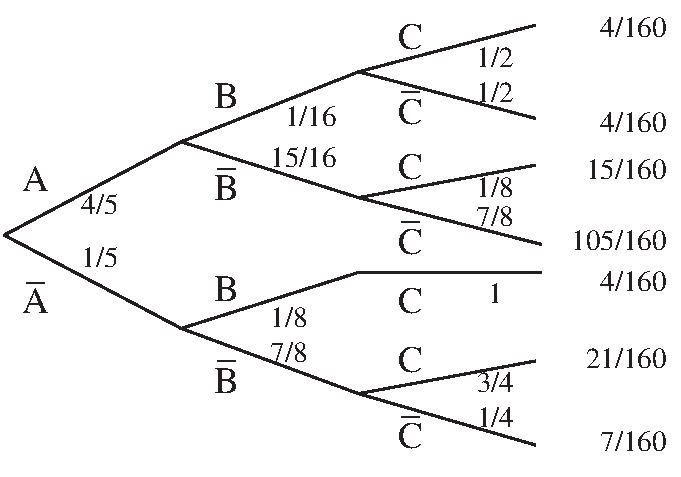
\includegraphics[scale=0.8]{figurer/fig4_3.pdf} 
\caption{Hansens sannsynligheter}
	\label{fig:hansens_sannsynligheter}
\end{figure}
Her er eksempelvis $P(A)=4/5$, $P(B\mid A)=1/16$ og $P(C\mid A \cap B)=1/2$.
 Ved å multiplisere sammen sannsynlighetene langs grenene
finner vi tallene til høyre for treet, eksempelvis er (jfr.
Oppgave~10):

\[ P(A\cap B\cap C)=P(A)\cdot P(B\mid A)\cdot P(C\mid A\cap B)
            =\frac{4}{5} \cdot \frac{1}{16} \cdot \frac{1}{2} = \frac{4}{160}\]

\noindent Vi finner at

\[ P(C) = \frac{4}{160} + \frac{15}{160} + \frac{4}{160}+\frac{21}{160} = \frac{11}{40} \]
\end{eksempel}
Et teoretisk grunnlag for subjektiv sannsynlighet er utviklet i
vårt århundre som en integrert del av generell beslutningsteori.
For en beslutningstaker som står overfor beslutninger under
usikkerhet kan man, ved å anta at han/hun oppfyller visse
adferdsforutsetninger, utlede at han/hun vil (bør) handle som om han/hun regnet
med sannsynligheter som følger de vanlige regnereglene for slike.
Disse sannsynlighetene vil ifølge sin natur måtte være
subjektive. Dette tema blir tatt opp til grundigere diskusjon i
Kapittel 16. \\[0.2cm]
          

\section{Uavhengige begivenheter}

La $A$ og $B$ være to begivenheter. Sannsynligheten for $A$ er
$P(A)$ (ubetinget), mens den betingede sannsynlighet for $A$ gitt
$B$ er $P(A\mid B)$. I enkelte si\-tua\-sjoner viser det seg at
begivenhetene $A$ og $B$ er slik at disse to sannsynlighetene er
like, dvs. at $P(A\mid B)=P(A)$. Dette kan tolkes slik at det
faktum at $B$ har inntruffet ikke påvirker sjansen for at $A$
skal inntreffe, og det er naturlig å si at begivenheten $A$ er
uavhengig av begivenheten $B$. På samme måte dersom $P(B\mid A) =
P(B)$ er det naturlig å si at $B$ er uavhengig av $A$.
Av E8, E9 og E10 følger det imidlertid at følgende tre utsagn er
ekvivalente (såframt $P(A)>0$ og $P(B)>0$)
\begin{itemize}
\item[(i)]                 $P(A\mid B)  = P(A)$
\item[(ii)]                $P(B\mid A)  = P(B)$
\item[(iii)]               $P(A\cap B)  = P(A) \cdot P(B)$
\end{itemize}
Siden det viste seg at uavhengighet er et symmetrisk begrep, er
det naturlig å velge en symmetrisk definisjon:
\begin{center} \framebox[10cm]{\begin{minipage}{9cm}\rule{0cm}{0.5cm}
\begin{definisjon}
      Begivenhetene $A$ og $B$ sies å være
     {\em uavhengige} dersom $P(A\cap B)=P(A)\cdot P(B)$
\end{definisjon}
  \end{minipage}} \end{center}

\begin{eksempel}{Korttrekning}
Et kort trekkes tilfeldig fra en kortstokk. La \\[3mm]
\indent     $A$ = Sort kort \\
\indent     $B$ = Honnør \\[3mm]
Her er $P(A)=1/2$, $P(B)=4/13$ og $P(A \cap B)=8/52=2/13$.
Vi ser at $P(A\cap B)=P(A)\cdot P(B)$, og vi har dermed vist at
begivenhetene $A$ og $B$ er uavhengige. Dette samsvarer vel med
vår intuisjon.
\end{eksempel}

\begin{eksempel}{To terningkast}
Anta en modell hvor alle $m = 36$ mulig utfall er like
sannsynlige, og la \\[3mm]
\indent     $E_i =$ første kast gir $i$ øyne,    $i = 1,2,\ldots,6$\\
\indent     $F_j =$ annet kast gir $j$ øyne,   $j = 1,2,\ldots,6$ \\[3mm]
Her er $P(E_i \cap F_j)=1/36$, mens $P(E_i)=6/36=1/6$ og $P(F_j)=6/36=1/6$.
Vi ser at $P(E_i \cap F_j)=P(E_i) \cdot P(F_j)$, slik at vi kan
konkludere med at $E_i$ og $F_j$ er uavhengige. Det kan vises at
dersom $E$ og $F$ er to vilkårlige begivenheter som refererer seg
til henholdsvis første og annet kast, så er de uavhengige. Vi sier
at de to kastene utgjør to {\em uavhengige deleksperimenter.}
\end{eksempel}

Vi har også bruk for begrepet uavhengighet for mer enn to
begivenheter:
\begin{center} \framebox[12cm]{\begin{minipage}{11cm}\rule{0cm}{0.5cm}
\begin{definisjon}
     De $n$ begivenheter $A_1, A_2, \ldots,
     A_n$ sies å være {\em uavhengige} dersom sannsynligheten for
     snittet av ethvert utvalg av disse begivenhetene er lik
     produktet av sannsynlighetene.
\end{definisjon}
  \end{minipage}} \end{center}
Vi merker oss f.\ eks.\ at dersom tre begivenheter $A$, $B$ og $C$
skal være uavhengige, så må
\begin{center}
\begin{enumerate}
\item        $P(A\cap B\cap C)=P(A)\cdot P(B)\cdot P(C)$ 
\item        $P(A\cap B)=P(A)\cdot P(B), P(A\cap C)=P(A)\cdot P(C)$,\\
             $P(B\cap C)=P(B)\cdot P(C)$
\end{enumerate}
\end{center}

I dagligtale, ikke minste i sport og spill, brukes ofte begrepet ``odds''.
En begivenhet $A$ har odds lik $O(A)=P(A)/P(\bar{A})$, mens for gitt $B$ 
er odds for $A$ endret til $O(A\mid B)=P(A\mid B)/P(\bar{A}\mid B)$.
I Eksempel 8 med gullfisken blir $O(A)=1:3$, mens $O(A\mid B)=5:3$ og
$O(A\mid \bar{B})=5:27$. Merk at uttrykt ved odds blir den tilhørende 
sannsynlighet $P=O/(1+O)$. I totalisatorspill betyr et tilbudt odds hvor 
mange ganger innsatsen spilleren får ved vinst.

Et mål for grad av avhengighet er det såkalte {\em odds-forholdet} 
med verdier mellom 0 og $\infty$:

\[    OR(A,B) = \frac{O(A\mid B)}{O(A\mid \bar{B})}=\frac{O(B\mid A)}{O(B\mid \bar{A})} \]
Dette er 1 hvis og bare hvis $A$ og $B$ er uavhengige, og større enn/mindre enn 1 
alt ettersom $A$ er mest sannsynlig sammen med $B$ eller $\bar B$.
Et alternativt mål er $G=(OR-1)/(OR+1)$, med verdi mellom -1 og +1, der 0
svarer til uavhengighet. 
I Eksempel 9 blir $OR(A,B)=5:3/5:27=1:1/1:9=9$, mens $G=(9-1)/(9+1)=0.8$. 

\section{Uavhengige eksperimenter og produkt\-modeller}

I forrige avsnitt så vi hvordan vi i en modell kunne sjekke om
begivenheter er uavhengige. I dette avsnitt skal vi se hvordan
begrepet uavhengighet kan brukes den motsatte veien til
konstruksjon av modeller: Har man forestillinger om at visse
begivenheter er uavhengige, er det naturlig at disse
forestillinger kommer til uttrykk i modellen.
I praksis støter en ofte på situasjoner hvor et eksperiment kan
betraktes som sammensatt av to eller flere deleksperimenter, som
man forestiller seg ikke avhenger av hverandre. Det er da
naturlig å anta at deleksperimentene er uavhengige, dvs. at en
samling begivenheter som hører til hvert sitt
deleksperiment er uavhengige.\\

\begin{eksempel}{To terningkast}
La oss som i Eksempel 11 definere \\[3mm]
\indent     $E_i =$ første kast viser i øyne \\
\indent     $F_j =$ annet kast viser j øyne \\[3mm]
Dersom hvert av kastene skjer med en rettferdig terning, er det
rimelig å sette
\[ P(E_i)=\frac{1}{6} \mbox{\ \  for \ \ } i=1,2, \ldots,6 \]
\[ P(F_j)=\frac{1}{6} \mbox{\ \  for \ \ } j=1,2, \ldots,6 \]
Antar vi at de to kastene er uavhengige, får vi

\[ P(E_i \cap F_j)=P(E_i) \cdot P(F_j)=\frac{1}{6} \cdot \frac{1}{6}
                             =\frac{1}{36} \]
Selv om dette gir oss den samme modell for de to kastene som den
vi hadde i Eksempel 12, er det viktig å merke seg den
prinsipielle forskjell: I Eksempel 12 startet vi med en
totalmodell for de to kastene og påviste at begivenheter
vedrørende hvert sitt kast var uavhengige. I Eksempel 13 starter
vi med sannsynligheter for begivenheter vedrørende hvert sitt
kast, og benytter så forestillingen om uavhengige kast til å
beregne sannsynligheten for begivenheter vedrørende begge kast.
For å illustrere at dette virkelig representerer et nytt
hjelpemiddel ved konstruksjon av sannsynlighetsmodeller, kan vi
se på to kast med en falsk terning: Anta at det (f. eks. på
bakgrunn av empirisk erfaring) er rimelig å sette \\

$P(E_1)=0.19,P(E_2)=P(E_3)=P(E_4)=P(E_5)=0.17,P(E_6)=0.13$ \\

\noindent og likeens \\

$P(F_1)=0.19,P(F_2)=P(F_3)=P(F_4)=P(F_5)=0.17,P(F_6)=0.13$ \\

\noindent Antar vi at de to kastene er uavhengige, får vi

%\begin{center}
\begin{tabular}{ccccccc}
 $P(E_1\cap F_1)$&$=$&$P(E_1)\cdot P(F_1)$&$=$&$0.19\cdot 0.19$&$=$&$0.0361$ \\
 $P(E_1\cap F_2)$&$=$&$P(E_1)\cdot P(F_2)$&$=$&$0.19\cdot 0.17$&$=$&$0.0323$ \\
 $P(E_2\cap F_2)$&$=$&$P(E_2)\cdot P(F_2)$&$=$&$0.17\cdot 0.17$&$=$&$0.0289$ \\
     $\vdots$     &   &   $\vdots$         &   &      $\vdots$   &   & $\vdots$ \\
 $P(E_6\cap F_6)$&$=$&$P(E_6)\cdot P(F_6)$&$=$&$0.13\cdot 0.13$&$=$&$0.0169$
\end{tabular}
%\end{center}
\end{eksempel}

\begin{eksempel}{Brannalarm}
Sannsynligheten for at en bestemt type brannalarm skal virke ved
brann er 0.9. Hva er sannsynligheten for alarm $(A)$ dersom man
installerer tre slike alarmer som virker uavhengig av hverandre?
La \\ \\
\indent  $A_i=$ Alarm nr. $i$ virker, $i=1,2,3$. \\ \\
\noindent Vi ser at \\ \\
\indent $A=A_1\cup A_2\cup A_3$  \ \ \ mens \ \ \
              $\bar{A}=\bar{A_1} \cap \bar{A_2} \cap \bar{A_3}$  \\ \\
Det at alarmene virker uavhengig av hverandre tolkes dithen at
 $\bar{A_1}$, $\bar{A_2}$ og $\bar{A_3}$ blir uavhengige begivenheter.
 Vi får derfor
 \begin{eqnarray*}
 P(A)&=&1-P(\bar{A})=1-P(\bar{A_1} \cap \bar{A_2} \cap \bar{A_3}) \\
     &=&1-P(\bar{A_1}) \cdot P(\bar{A_2}) \cdot P(\bar{A_3}) \\
     &=&1-0.1^3=1-0.001=0.999 
\end{eqnarray*}
\end{eksempel}

\begin{eksempel}{Myntkast inntil første kron}
La oss for $i=1,2,3,\ldots$ definere \\ \\
\indent     $A_i=$ Kast nr. $i$ er mynt \\ \\
Med en rettferdig mynt setter vi $P(A_i)=\frac{1}{2}$  for
$i=1,2,\ldots$.
La $B_n=$ første kron inntreffer i n'te kast. Vi får

\[  B_n=A_1\cap A_2\cap \cdots \cap A_{n-1}\cap \bar{A_n} \]
Antar vi at kastene er uavhengige, får vi
\begin{eqnarray*}
 P(B_n)&=&P(A_1\cap A_2\cap \cdots \cap A_{n-1}\cap \bar{A_n}) \\
       &=&P(A_1)\cdot P(A_2)\cdots P(A_{n-1}) \cdot P(\bar{A_n}) \\
       &=&\frac{1}{2} \cdot\frac{1}{2} \cdots \frac{1}{2} 
                  \cdot \frac{1}{2}={(\frac{1}{2})}^n
\end{eqnarray*}
\noindent et resultat som ble annonsert i Eksempel 2.12.
\end{eksempel}
En modell konstruert som i eksemplene ovenfor kalles en {\em
produktmodell}. Det kreves egentlig en formell begrunnelse for at
dette kan gjøres på en logisk konsistent måte. 
Vi antyder dette som $\star$-merket stoff.\\

\small
 
$\star$ Gitt et eksperiment som består av to deleksperimenter. 
Anta at en brukbar modell for første eksperiment er gitt ved:

\begin{center}
\begin{tabular}{lccccl}
Mulige utfall:  &  $e_1$&$e_2$&$\ldots $&$e_m$& \\
Sannsynligheter:&  $p_1$&$p_2$&$\ldots $&$p_m$&slik at\ \ $\sum_{i=1}^{m}p_i=1$
\end{tabular}
\end{center}
mens en brukbar modell for annet eksperiment er gitt ved :
\begin{center}
\begin{tabular}{lccccl}
Mulige utfall:  & $f_1$&$f_2$&$\ldots $&$f_n$& \\
Sannsynligheter:& $q_{1}$&$q_{2}$&$\ldots $&$q_{n}$&slik at\ \ $\sum_{j=1}^{n}q_{j}=1$
\end{tabular}
\end{center}
En modell for hele eksperimentet bruker utfallsrommet:
\begin{center}
\begin{tabular}{rccccc}
    $\Omega =$&$\{(e_1, f_1),$&$(e_1, f_2),$&$\ldots$,&$(e_1, f_n),$ \\
              &$  (e_2, f_1),$&$(e_2, f_2),$&$\ldots$,&$(e_2, f_n),$ \\
              &        .     &       .     &       &       .      \\
              &        .     &       .     &       &       .      \\
              &        .     &       .     &       &       .      \\
              &$(e_m, f_1),$&$(e_m, f_2),$&$\ldots$,&$(e_m, f_n)\}$ 
\end{tabular}
\end{center}
Antar vi at de to deleksperimentene er uavhengige, er det rimelig å
tildele utfallet $(e_i,f_j)$ en sannsynlighet lik produktet av de
faktorene \\ 

      $P((e_i, f_j))=p_iq_{j}$ \ $i=1,2,\ldots ,m,\; j=1,2,\ldots ,n$. \\

\noindent Vi ser at dette definerer en sannsynlighetsmodell, fordi \\

 $    \sum_{i} \sum_{j} P((e_i,f_j))=\sum_{i} \sum_{j} p_iq_{j}
        =(\sum_{i} p_i) \cdot (\sum_{j}q_{j})= 1 \cdot 1=1 $ \\

Det overlates til leseren å sjekke at sannsynlighetene fra 
deleksperimentene kan gjenvinnes på en konsistent måte fra
totalmodellen. og at konstruksjonen kan utvides til et vilkårlig
antall deleksperimenter. Vanskelig blir dette først når denne
id\'{e}en skal generaliseres til utfallsrom som ikke er endelige.
Det var slike grunnleggende problemer sann\-syn\-lig\-hets\-teo\-re\-tikere
ryddet opp i på 1900-tallet.

\normalsize

\section{Binomiske forsøksrekker}

Mange praktiske problemstillinger kan tilbakeføres til følgende
situasjon:
\begin{center} \framebox[12cm]{\begin{minipage}{10cm}\rule{0cm}{0.5cm}
 {\bf Binomisk forsøksrekke}. 
Det utføres en rekke forsøk (eksperimenter, iakttakelser), der 
\begin{enumerate}
\item Hvert forsøk resulterer enten i suksess (S) eller fiasko
     (F).
\item Sannsynligheten for suksess er den samme i alle forsøk.
\item Forsøkene er uavhengige.
\end{enumerate} \mbox{}
  \end{minipage}} \end{center}
Anta at vi utfører $n$ binomiske forsøk og la oss betegne
sannsynligheten for suksess i hvert forsøk med $p$. Vi ønsker nå
å beregne sannsynligheten for at vi i løpet av de $n$ forsøkene
observerer $X$ suksesser:
Siden forsøkene er uavhengige blir sannsynligheten for utfallet
\[  SS\cdots SFF \cdots F \]
\noindent dvs. først $x$ suksesser og deretter $n-x$ fiaskoer lik

\[ p\cdot p\cdots p\cdot (1-p)\cdots (1-p)=p^x(1-p)^{n-x} \]

\noindent På tilsvarende måte blir sannsynligheten for ethvert annet
spesifisert utfall bestående av $x$ suksesser og $n-x$ fiaskoer
også lik $p^x(1-p)^{n-x}$ (faktorenes orden er likegyldig). Siden
det er $\bino{n}{x}$ måter å velge ut de $x$ forsøkene som skal gi
suksess, er det $\bino{n}{x}$ gunstige utfall for begivenheten at vi
får $x$ suksesser, og hvert av disse  har sannsynlighet $p^x(1-
p)^{n-x}$. Følgelig blir sannsynligheten for $x$ suksesser i
løpet av de $n$ forsøkene lik
\[ \bino{n}{x}p^x(1-p)^{n-x} \]
\noindent Denne formelen gjelder for $x=0,1,2,\ldots,n$.\\

\begin{eksempel}{Ti myntkast}
Dette kan betraktes som en binomisk forsøksrekke med $n=10$
forsøk, hvor kron tilsvarer suksess. Antar vi rettferdig mynt får
vi at sannsynligheten for i alt $x$ kron i løpet av de ti
myntkastene blir

\[ \bino{10}{x}{(\frac{1}{2})}^x{(1-\frac{1}{2})}^{10-x}=
          \bino{10}{x}{(\frac{1}{2})}^{10}  \]

\noindent Eksempelvis blir sannsynligheten for bare 3 kron
\[       \bino{10}{3}{(\frac{1}{2})}^{10}=\frac{120}{1024}  \]
\end{eksempel}
        
\begin{eksempel}{Ti terningkast}
La oss anta at sekser betyr suksess. Situasjonen kan betraktes
som en binomisk forsøksrekke med $n=10$ forsøk og med 
suksess-sannsynlighet 1/6. Sannsynligheten for $x$ seksere i løpet av de
ti kastene blir
\[ \bino{10}{x}{(\frac{1}{6})}^x{(1-\frac{1}{6})}^{10-x}  \]
\noindent Eksempelvis blir sannsynligheten for 7 seksere
\[ \bino{10}{7}{(\frac{1}{6})}^7{(1-\frac{1}{6})}^3  \]
\noindent mens sannsynligheten for minst 7 seksere blir
\[ \sum_{x=7}^{10}\bino{10}{x}{(\frac{1}{6})}^x{(1-\frac{1}{6})}^{10-x}  \]
\end{eksempel}

\begin{eksempel}{Produksjonsprosess}
En produksjonsserie består av $n=100$ artikler. Hver artikkel
klassifiseres som enten defekt eller intakt. Anta at for hver
artikkel så er sannsynligheten for at den er defekt lik 0.05.
Anta videre uavhengighet. Vi har dermed en binomisk
forsøksrekke. Sannsynligheten for $x$ defekte artikler i
produksjonsserien blir

\[ \bino{100}{x}{0.05}^x{(1-0.05)}^{100-x}  \]

\noindent Eksempelvis blir sannsynligheten for 5 defekte
\[ \bino{100}{5}{0.05}^5{0.95}^{95}  \]         
\noindent mens sannsynligheten for høyst 5 defekte blir
\[ \sum_{x=0}^{5} \bino{100}{x}{0.05}^x{0.95}^{100-x}  \]
\end{eksempel}

Det finnes tabeller over binomiske sannsynligheter, som vil
redusere det praktiske regnearbeid ved beregning av slike, se
Tabell~\ref{tab:Binomisk_fordeling} og~\href{tab:Binomisk_fordeling_p05} 
i Appendiks~\ref{app:fordelngstabeller}. Vi vil ta opp binomiske forsøk til
bredere diskusjon i Kapittel 6.2, og en nærmere veiledning i
bruken av tabeller utstår til da.
En annen interessant problemstilling i forbindelse med binomiske
forsøksrekker er å finne sannsynligheten for at første suksess
kommer i n'te forsøk. I en situasjon hvor en observerer en
binomisk forsøksrekke inntil første suksess kan det være
hensiktsmessig å tenke seg de mulige utfall i utfallsrommet
$\Omega$ som

\[ S,\;\; FS,\;\; FFS,\;\; FFFS, \ldots \]
dvs. første suksess i første forsøk, første suksess i annet
forsøk etc. Siden forsøkene er antatt å være uavhengige betyr det
at disse utfallene tildeles sannsynlighetene

\[ p,\;\; (1-p)p,\;\; (1-p)(1-p)p,\;\; (1-p)(1-p)(1-p)p, \ldots  \]
med andre ord sannsynligheten for at første suksess kommer i n'te
forsøk blir derfor

\[   (1-p)^{n-1} \cdot p   \mbox{\ \ \ for \ \ } n=1,2,3, \ldots  \]

\noindent Ved å benytte summeformelen for en geometrisk rekke, ser vi at
disse sannsynlighetene summerer seg opp til en, slik at vi dermed
har fått etablert en sannsynlighetsmodell. Legg merke til at
dette innebærer at sannsynligheten for at vi observerer i det
uendelige uten å få suksess er null, dette utfallet er følgelig
heller ikke tatt med som et mulig utfall. Sannsynligheter av
typen ovenfor blir gjerne kalt for {\em geometriske sannsynligheter}.

Vi har sett eksempel på slike sannsynligheter i Eksempel 15 hvor
problemet var ventetiden til første kron i myntkast
 \footnote{I dette eksemplet brukte vi riktignok en annen men likeverdig
formalisering ved løsningen av problemet, vi ønsker å få vist
begge.}, i dette tilfellet er  $p$=1/2 . Et annet eksempel vil
være ventetiden til første sekser i terningkast, i dette
tilfellet er $p=1/6$. Sannsynligheten for at første sekser kommer
i n'te kast er derfor

\[ {(\frac{5}{6})}^{n-1} \cdot \frac{1}{6} 
                            \mbox{\ \ \ for \ \  } n=1,2,3, \ldots  \]
Enda et eksempel vil være ventetiden til første defekte artikkel
i en produksjonsprosess som gjennomgående i det lange løp gir 5\%
defekte. Dersom vi antar uavhengighet med hensyn til defekt og
intakt for de ulike produksjonsnumre, vil også denne situasjon
falle innenfor rammen av teorien ovenfor, nå med $p=0.05$.
Sannsynligheten for at første defekt kommer som produksjonsnummer
$n$ er derfor:

\[  0.95^{n-1} \cdot 0.05   \mbox{\ \  for \ \  } n=1,2,3, \ldots  \]
Vi vil komme tilbake til geometriske sannsynligheter i Kapittel 6.7.
               
\section{$\star$Paradokser}
\small
Sannsynlighetsregning rommer en rekke paradokser som kan ha
praktiske konsekvenser. Vi gir her to eksempler
på statistiske problemstillinger med fare for feilkonklusjoner,
der innsikt i betingede sannsynligheter kan klargjøre situasjonen.\\

\begin{eksempel}{Representasjonsfellen}
Betrakt følgende utsagn
\begin{quote}
``Folkegruppe B utgjør 10 \% av befolkningen, men utgjør 15\% av
dem som har et bestemt gode''.
\end{quote}
Utsagnet inviterer leseren til å konkludere at folkegruppe $B$ er
favorisert, noe som kan være forhastet.  Fellen kan lett blottlegges
ved betraktninger rundt betingede sannsynligheter.

La $A$ være begivenheten at en tilfeldig person i befolkningen har godet.
Det vil være relevant å sammenligne $P(A\mid B)$ for ulike 
folkegrupper, men utsagnet ovenfor sammenligner i stedet $P(B \mid A)$ med
$P(B)$.  Dersom $P(B \mid A)$ er større (mindre) enn $P(B)$, kan vi ikke
slutte mer enn at $P(A \mid B)$ er større (mindre) enn den tilsvarende 
sannsynlighet for minst en annen gruppe $B$.

La oss ta et talleksempel begrenset til tre grupper $B_1$, $B_2$ og $B_3$,
og la sannsynlighetene for at en tilfeldig person tilhører hver av gruppene
være
\begin{eqnarray*}
  P(B_1) = 0.40  &   P(B_2) = 0.10  &   P(B_3) = 0.50    
\end{eqnarray*}
Anta videre at betingede sannsynligheter $P(A \mid B_i)$ er gitt ved to
situasjoner i tabellen nedenfor, og at vi fokuserer på $B_2$.  Vi beregner
derfor $P(B_2 \mid A)$ ved Bayes lov (sjekk beregningen).
\begin{center}
\begin{tabular}{l|ccc|c}
    &$P(A \mid B_1)$&$P(A \mid B_2)$&$P(A \mid B_3)$ &$P(B_2 \mid A)$\\ \hline
Situasjon 1 &       0.1    &       0.5      &      0.6      &    0.14  \\
Situasjon 2 &       0.1    &       0.2      &      0.6      &    0.06
\end{tabular}
\end{center}
Vi ser at i situasjon 1 kommer gruppe 2 godt ut ved sammenligningen 
$0.14 > 0.10$, mens det i virkeligheten fins en langt større gruppe ($B_3$)
som er bedre stillet, men også en gruppe ($B_1$) som er dårligere
stillet.  Kommenter selv situasjon 2. 
\end{eksempel}

Utsagn som er beslektet med det som er gitt i eksemplet forekommer ofte i
media, oftest ubevisst, men er også brukt bevisst i meningspåvirkning.
Eksempler på situasjoner:
diskriminering mellom folkegrupper,
sykdomsforekomst i ulike sosialgrupper,
uhellsforekomst i ulike grupper (f.eks. av bilister),
reklame og politisk kampanjevirksomhet og
forbrukerspørsmål, f.eks. produktansvar.
\mbox{} \\

\begin{eksempel}{Diskriminering?}
Betrakt følgende medieoppslag :
\begin{quote}
``Ved høstens opptak tok UCB-universitetet opp 44 \% av de mannlige 
søkere og 35 \% av de kvinnelige.''
\end{quote}
Dette kunne skyldes at andelen kvinner med dårlig opptaksgrunnlag 
var større enn blant de mannlige. Dersom det kan godtgjøres at
dette var likelig fordelt, er det vel grunnlag for å hevde at
diskriminering har funnet sted? Ikke ubetinget!
Anta at opptak skjer ved søknad til de enkelte institutter.
I et forsøk  på å finne ut hvilke som eventuelt diskriminerer,
viste det seg at ingen gjorde det. Andelen opptatte kvinner var omtrent
lik mennenes ved de fleste, og ved et par institutter var andelen opptatte 
kvinner faktisk større. Forklaringen på dette tilsynelatende
paradoks var at kvinnene hadde i større utstrekning søkt til
institutter der det var vanskelig å komme inn.
\end{eksempel}
Den beskrevne situasjon er et eksempel på det såkalte 
{\em Simpson's paradoks}. En formulering i sannsynlighetsteoretiske termer
kan bidra til å klargjøre dette.
\begin{center} \framebox[11cm]{\begin{minipage}{10cm}\rule{0cm}{0.5cm}
{\bf Simpson's paradoks : } \\
La $\Omega = B_1 \cup B_2 \cup \ldots \cup B_r$ være en disjunkt
oppsplitting av den sikre begivenhet. Anta at
\[ P(C\mid A\cap B_i) \geq P(C\mid \bar{A}\cap B_i) \mbox{\ \ for alle i} \]
Det er likevel mulig atP$(C\mid A) < P(C\mid \bar{A})$.
\mbox{} \end{minipage}} \end{center}
La oss i Figur~\ref{fig:simpsons_paradoks} illustrere at dette er mulig i den enkleste situasjonen der
$\Omega = B\cup \bar{B}$.

\begin{figure}[ht]
\centering \centering
 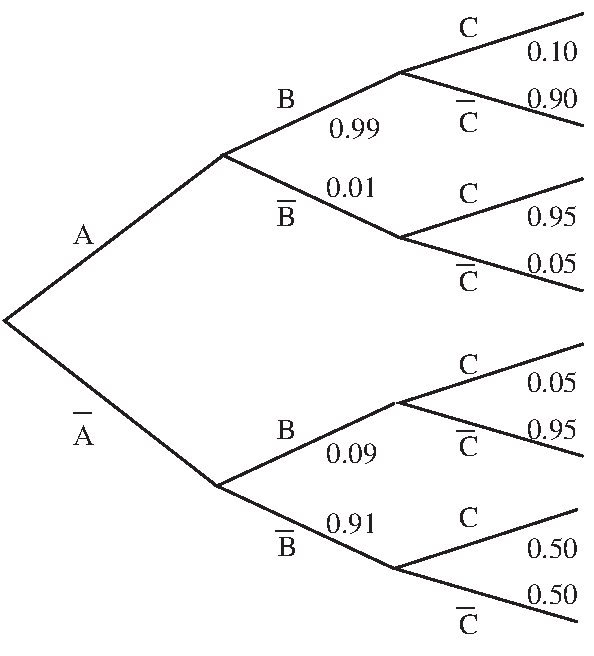
\includegraphics[scale=0.7]{figurer/fig4_4.pdf} 
 \caption{Simpsons paradoks}
	\label{fig:simpsons_paradoks}
\end{figure}

Her er betingelsen oppfylt, mens
\begin{eqnarray*}
P(C\mid A)&=&P(B\mid A) \cdot P(C\mid A\cap B)
                +P(\bar{B}\mid A) \cdot P(C\mid A\cap \bar{B}) \\
          &=&0.99 \cdot 0.10 + 0.01 \cdot 0.95 = 0.11 \\
P(C\mid \bar{A})&=&P(B\mid \bar{A}) \cdot P(C\mid \bar{A}\cap B)
                +P(\bar{B}\mid \bar{A}) \cdot P(C\mid \bar{A}\cap \bar{B}) \\
          &=&0.09 \cdot 0.05 + 0.91 \cdot 0.50 = 0.46 
\end{eqnarray*}
For å knytte forbindelsen til eksemplet over, la $C$=opptatt,
$B_i$=søker til institutt nr.i og $A$=kvinnelig søker.
\mbox{} \\

Simpson's paradoks opptrer i mange forkledninger, og det gjelder å
være på vakt! Greier du denne :  Er det mulig at totalbeskatningen
er øket fra et år til et annet, mens beskatningen i alle
inntektsgrupper har gått ned?

\section{$\star$Pålitelighetsanalyse}
\small
Sannsynlighetsregning har de senere år i stigende grad blitt tatt i
bruk ved studier av systempålitelighet. Vi gir her tre enkle eksempler,
hver med sin egen form for systembeskrivelse, henholdsvis
{\em logisk diagram}, {\em begivenhetstre} og {\em feiltre}.\\

\begin{eksempel}{Systempålitelighet : Logisk diagram}
Betrakt  følgende enkle situasjon, der vi har en strømkilde og to
radiosendere. For å sende signal må strømkilden og minst en av
senderne virke. Dette er illustrert i diagrammet i Figur~\ref{fig:logisk_diagram} med
sannsynligheter påført hver enhet for at den virker.

\begin{figure}[ht]
\centering\centering
 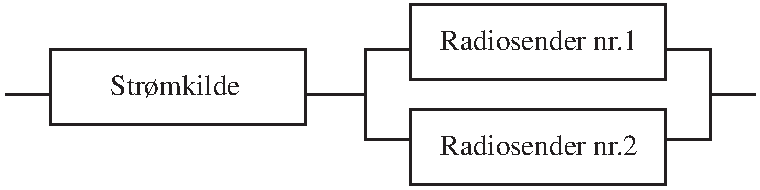
\includegraphics[scale=0.8]{figurer/fig4_5.pdf}
\caption{Logisk diagram}
	\label{fig:logisk_diagram}
\end{figure}

Anta at enhetene virker/ikke virker uavhengig av hverandre. Da blir
\begin{eqnarray*}
 P(S \cap (B_1 \cup B_2)) &=& P(S) \cdot P(B_1 \cup B_2) \\
                          &=& P(S) \cdot (P(B_1)+P(B_2)-P(B_1 \cap B_2) \\
                          &=& P(S) \cdot (P(B_1)+P(B_2)-P(B_1) \cdot P(B_2)) \\
                          &=& 0.999 \cdot (0.99+0.99-0.99 \cdot 0.99) \\
                          &=& 0.999 \cdot 0.9999=0.9989
\end{eqnarray*}
\end{eksempel}
\begin{eksempel}{Systempålitelighet : Begivenhetstre}
En begivenhet $B$ som representerer et uhell, f.eks. brann, utløser
aktiviteter for å bringe situasjonen under kontroll, f.eks. bruk av
brannslokningsutstyr. Anta at situasjonen er som beskrevet i
begivenhetstreet i Figur~\ref{fig:begivenhetstre}. 

\begin{figure}[ht]
\centering \centering
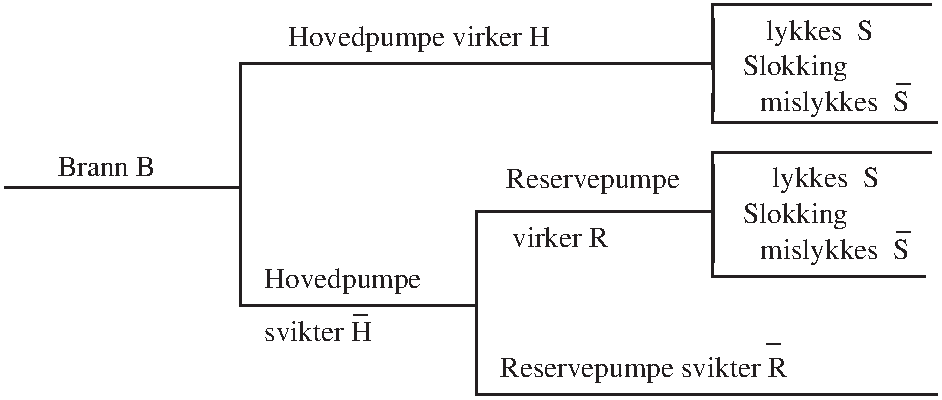
\includegraphics[scale=0.7]{figurer/fig4_6.pdf} 
\caption{Begivenhetstre}
	\label{fig:begivenhetstre}
\end{figure}

Sannsynligheten for at brann oppstår som ikke slokkes ($A$) blir da
\begin{eqnarray*}
P(A)&=&P(B) \cdot P(H \mid B) \cdot P(\bar{S} \mid B \cap H) \\
    &+&P(B) \cdot P(\bar{H} \mid B) \cdot P(R \mid B \cap \bar{H})
                 \cdot  P(\bar{S} \mid B \cap \bar{H} \cap R) \\
    &+&P(B) \cdot P(\bar{H} \mid B) \cdot P(\bar{R} \mid B \cap \bar{H})
\end{eqnarray*}
Kompliserte systemer vil omfatte mange muligheter for feil eller uhell,
og hver kan tenkes analysert på tilsvarende måte, ofte med
forenklende antakelser om uavhengighet. Sannsynligheten for feil/uhell
av et eller annet slag i tidsperioden beregnes oftest ved å summere
enkeltsannsynlighetene, fordi dette i hvert fall ikke undervurderer
totalsannsynlighetene (hvorfor?). En må imidlertid alltid stille
spørsmålene
\end{eksempel}
% HJS: her har jeg flyttet ``itemize" utenfor ekspemplelet pga kompileringsfeil
\begin{itemize}
\item Er alle tenkelige uhellstyper tatt med?
\item Er enkeltsannsynlighetene realistiske?
\item Er evt. forenklende antakelser om uavhengighet realistiske? 
\end{itemize}
\mbox{} \\

\begin{eksempel}{Systempålitelighet : Feiltre}
Ofte studeres de betingelser som må være tilstede for at uhell skjer,
noe som ofte kan beskrives ved et feiltre som beskrevet i Figur~\ref{fig:feiltre}.

\begin{figure}[ht]
\centering\centering
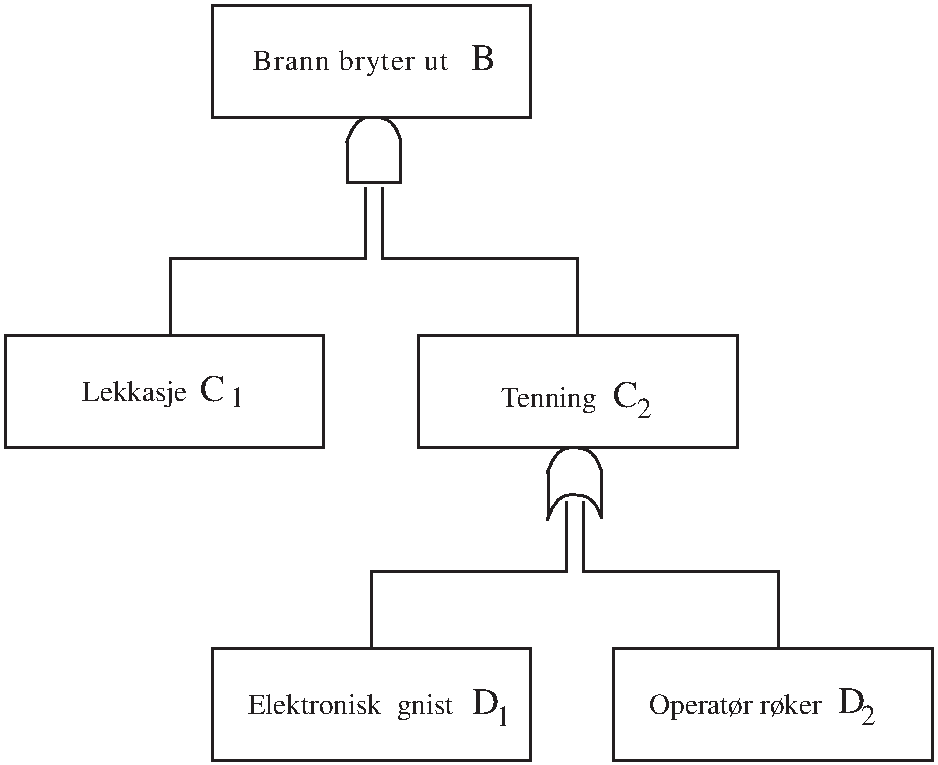
\includegraphics[scale=0.6]{figurer/fig4_7.pdf} 
\caption{Feiltre}
	\label{fig:feiltre}
\end{figure}

Legg merke til at dette er tilbakeskuende, mens begivenhetstreet ser forover.
Vi ser at
\begin{eqnarray*}
P(B)&=&P(C_1) \cdot P(C_2) \\
    &=&P(C_1) \cdot P(D_1 \cup D_2) \\
    &\approx&P(C_1) \cdot (P(D_1)+P(D_2))
\end{eqnarray*}
\end{eksempel}
\normalsize

\section{Oppgaver}
\small
\begin{enumerate}
	\item   I Oppgave~\ref*{kap:diskrete}.10-11 finn følgende betingede modeller (i)
     gitt $A$ (ii) gitt $B$ (iii) gitt $C$. Finn deretter  \\
     $P(A\mid B)$, $P(A\mid C)$, $P(B\mid A)$, $P(C\mid A)$,     
     $P(A\mid \bar{B})$, $P(A\mid \bar{C})$ og $P(C\mid \bar{A})$.
     Finn også  $P(A\mid A \cup B)$,  $P(A\mid A \cup C)$,
     $P(A\mid A \cap B)$,  $P(A\mid A \cap C)$,
     $P(A\mid A \cup \bar{C})$, $P(A\mid A \cap \bar{C})$,
     $P(A \mid \bar{A} \cap C)$ og $P(A \mid \bar{A} \cup B \cup C)$. 
     Kommenter.

\item   I Oppgave~\ref*{kap:diskrete}.12 finn sannsynlighetene $P(A\mid B)$, $P(B\mid
     A)$, $P(C\mid A)$ og $P(A\mid C)$. Kommenter.

\item   I Oppgave~\ref*{kap:diskrete}.18 finn $P(B\mid C), P(C\mid B), P(B\mid D),
     P(D\mid B)$.

\item   Regn ut noen betingede sannsynligheter etter eget valg for
	situasjonene i Oppgave~\ref*{kap:kombinatorikk}.16 og~\ref*{kap:kombinatorikk}.17.

\item  Anta at $P(A) = 0.3, P(B) = 0.2$ og $P(A \cup B) = 0.4$.
     Finn $P(A\mid B)$ og $P(B\mid A)$.

\item  I Oppgave~\ref*{kap:kombinatorikk}.25 finn den betingede sannsynligheten for minst
     en førsteklassing gitt minst en gutt på trinn 3 eller
     lavere.

\item   For situasjonen i Oppgave~\ref*{kap:kombinatorikk}.27 finn de betingede
     sannsynligheter for\\
     (a)  4 honnører gitt bare røde kort,\\
     (b)  bare røde kort gitt 4 honnører,\\
     (c)  ett ess gitt bare røde kort,\\
     (d)  ett ess gitt 4 honnører,\\
     (e)  4 honnører gitt et ess.\\
     Er noen av begivenhetene som omtales i Oppgave~\ref*{kap:kombinatorikk}.26
     uavhengige ?

\item  Vis at dersom $A\subset B$ så er
\[   P(A \mid B)=\frac{P(A)}{P(B)}  \]

\item   Vis at dersom $A$ og $B$ er disjunkte så er
\[   P(A \mid A \cup B)=\frac{P(A)}{P(A)+P(B)}  \]

\item  Vis at $P(A\cap B\cap C) = 
       P(A)\cdot P(B\mid A)\cdot P(C\mid A\cap B)$ \\
     Hint: Bruk E9 to ganger.

\item  Et parti på 26 artikler blir undersøkt ved en
     inspeksjonsplan som foregår i to trinn: Først trekkes
     tilfeldig 8 artikler. Dersom en eller flere er defekte
     forkastes hele partiet. Dersom alle er i orden trekkes 8 nye
     artikler tilfeldig fra de resterende i partiet og partiet
     forkastes dersom en eller flere av disse er defekte. Finn
     sannsynligheten for å akseptere et parti med 3 defekte.

\item  I spillet Russisk Rulett velger spilleren tilfeldig en av
     tre revolvere, hver med 5 kamre. Antall tomme kamre er
     henholdsvis 4, 3 og 2. Kamrene snurres rundt og revolveren
     avfyres mot tinningen. Hva er sannsynligheten for at
     spilleren overlever spillet? Gitt at han overlevet, hva er
     sannsynligheten for at skuddet ble avfyrt med den revolver
     med flest tomme kamre?

\item  Sannsynligheten for at en gift mann har sett et bestemt
     teaterstykke er 0.4, mens sannsynligheten for at en gift
     kvinne har sett stykket er 0.5. Sannsynligheten for at konen
     har sett stykket gitt at mannen har sett det er 0.9.
     For et vilkårlig valgt ektepar finn sannsynligheten for at \\
     (a)  begge ektefeller har sett stykket,\\
     (b)  mannen har sett stykket gitt at konen har sett det,\\
     (c)  minst en av ektefellene har sett stykket.
                
\item  En bedrift har to maskiner A og B som kan brukes til å
     produsere samme artikkel. A står for 80\% av produksjonen,
     mens B står for 20\%. Man har erfart at A leverer
     gjennomgående 5\% defekte, mens B leverer 1\% defekte. Hva er
     sannsynligheten for at den skriver seg fra maskin A?

\item  Anta at sannsynligheten for at Per vil leve om 20 år er 0.6,
     mens sannsynligheten for Pål er 0.9. Finn sannsynligheten for  \\
     (a)  begge lever,\\
     (b)  ingen lever,\\
     (c)  minst en lever.

\item  Det foreligger to urner, hver med 6 kuler. Urne nr. 1 har 4
     hvite og 2 sorte kuler, mens Urne nr. 2 har 3 hvite og 3
     sorte kuler. En urne velges tilfeldig og to kuler trekkes
     tilfeldig fra denne, begge var hvite. Hva er sannsynligheten
     for at kulene kommer fra Urne nr. 1 når \\
     (a)  trekningen skjer med tilbakelegging,\\
     (b)  uten tilbakelegging.

\item  I en ``multiple choice'' test er det $n$ svaralternativer
     for hvert spørsmål. Anta at sannsynligheten for at Per vet
     svaret på et bestemt spørsmål er $p$. Dersom han ikke vet
     svaret, antar vi at han krysser av tilfeldig. Hva er
     sannsynligheten for at Per visste svaret gitt at han krysset
     av riktig?

\item  La situasjonen være som beskrevet i Eksempel 10. Finn
     sannsynlighetene for \\
     (a)  veien stengt gitt for sent fremme,\\
     (b)  uhell underveis gitt for sent fremme,\\
     (c)  veien åpen gitt tidsnok fremme og intet uhell
     underveis.

\item  Lag et sannsynlighetstre i hver av følgende situasjoner \\
     (a) Eksempel 5,\mbox{\ \ }(b) Eksempel 6,\mbox{\ \ }(c) Eksempel 9.

\item  Per knipser to rettferdige mynter. Gitt at minst en viste
     kron. Hva er sannsynligheten for at begge viste kron?
     Løs oppgaven under forutsetningene \\
     (a)  Per ser resultatet av begge myntene, men gir deg     
     ufullstendig informasjon. \\
     (b)  Den ene mynten trillet tilfeldigvis under sofaen. \\
     Blir svaret det samme for (a) og (b)?

\item  Tre fanger A, B og C blir informert om at en av dem er valgt
     ut tilfeldig for å bli henrettet, mens de to andre blir satt
     fri. Fange A spør vokteren om han ikke i hemmelighet kan
     fortelle hvem av de to medfangene som skal settes fri,
     siden han allerede vet at en av disse skal settes fri.
     Vokteren nekter å svare fordi han mener at når A vet hvem av
     kameratene som blir satt fri, vil hans egen sjanse for å bli
     henrettet øke fra 1/3 til 1/2 fordi A nå er en blant to
     fanger hvorav en skal henrettes. Hva mener du om vokterens
     argumentasjon?

\item  En person er anholdt som mistenkt for en bestemt
     forbrytelse. Man venter på rapport fra kriminalteknisk
     laboratorium angående blodspor på åstedet. På grunnlag av
     det foreliggende bevismateriale vurderer inspektør Snusen at
     (apriori) sannsynligheten for at anholdte er skyldig er lik
     p. Beskjed kommer så om at anholdtes blodtype samsvarer med
     blodsporene på åstedet som stammer fra gjerningsmannen. Anta
     at andelen av befolkning som har denne blodtypen er lik r.
     Finn (aposteriori) sannsynligheten for at anholdte er
     skyldig uttrykt ved p og r.

\item  En rettferdig mynt knipses to ganger. La \\
     \indent      A = første kast viser kron, \\
     \indent      B = annet kast viser kron, \\
     \indent      C = kastene viser samme resultat.\\
     Er A og C uavhengige begivenheter? Enn B og C? Er A, B og C
     uavhengige?

\item  Vis at dersom A og B er uavhengige, så er også A og $\bar{B}$  
     uavhengige.

\item  En arbeider skal opplæres til å utføre en vanskelig
     arbeidsoperasjon. Man har erfart at 10\% av nye arbeidere
     greier å utføre operasjonen tilfredsstillende i første
     forsøk, 20\% i andre forsøk og 30\% i tredje forsøk. Anta
     uavhengighet mellom forsøkene og finn sannsynligheten for en
     ny arbeider i løpet av 3 forsøk vil lykkes \\
     (a)  alle tre ganger,\mbox{\ \ } (b)  ingen ganger,\\
     (c)  minst en gang,\mbox{\ \ \ }  (d)  akkurat en gang.

\item La situasjonen være som i forrige oppgave, men anta at 25\%
     av de nye arbeiderne har lært arbeidsoperasjonen i sitt
     tidligere arbeid, for disse er det 80\% sjanse for at de
     lykkes i hvert av de tre forsøkene. Finn sannsynlighetene
     for begivenhetene i (a), (b), (c) og (d) for en ny arbeider
     når vi ikke vet noe om hans tidligere arbeidsbakgrunn.

\item  Per har fått 8 kroner for å kjøpe et brød, men er falt for
     fristelsen å kjøpe en tyggegummi til 1 krone. For å ``redde''
     situasjonen har han funnet en venn som er villig til å
     knipse mynt og krone. Innsatsen er 1 krone i første omgang,
     taper Per, dobles innsatsen og slik fortsetter man inntil
     Per enten har vunnet tilbake den krona som gikk til tyggegummi,
     eller blitt blakk. Hva er sannsynligheten for at Per kommer
     hjem med brød?

\item  Et spill mellom to spillere består av spilleomganger, den
     som først vinner fire omganger vinner spillet. Anta at
     sannsynligheten for at A vinner første omgang er 1/2, og at
     i derpå følgende omganger er oddsene 2:1 i favør av den som
     vant siste omgang. Finn sannsynligheten for at A vinner etter \\
     (a)  etter 4 omganger,\mbox{\ \ } (b)  etter 5 omganger,\mbox{\ \ }
     (c)  før eller senere.

\item  En bedrift bruker en maskin som alltid justeres ved ukeslutt
     (5 dagers uke), men kan kreve ekstra justering i løpet av
     uken, som foretas etter endt arbeids\-dag. Man har erfart at
     maskinen på en dag da det er henholdsvis 1, 2, 3, 4 dager
     siden den ble justert sist, vil trenge ny justering ved
     arbeidsdagens slutt med sannsynligheter henholdsvis 0.10,
     0.12, 0.15, 0.20. Finn sannsynligheten for\\
     (a)  ingen ekstra justering i løpet av uken,\\
     (b)  første justering skjer på onsdag,\\
     (c)  justering må foretas på onsdag,\\
     (d)  justering ble foretatt på onsdag gitt at det var minst
          en ekstra justering.

\item Løs foregående oppgave dersom vi isteden antar at
      sannsynligheten er 0.10 for at maskinen krever justering etter endt 
      arbeidsdag uavhengig av hvor lenge det er siden den justert sist.

\item  $\star$I en bedrift er det 3 avdelinger, i avd. 1 er det 6 kvinner,
     3 menn, i avd. 2 er det 4 kvinner, 8 menn og i avd. 3 er det
     3 kvinner og 9 menn. To av de ansatte skal sendes på et kurs
     og man ønsker ikke at begge skal sendes på et kurs og man
     ønsker ikke at begge skal komme fra samme avdeling. Derfor
     velges først tilfeldig hvilke to avdelinger som skal være
     representert, deretter velges en representant tilfeldig fra
     hver av de utvalgte avdelingene. Finn sannsynligheten for at \\
     (a)  begge kursdeltakere er kvinner,\\
     (b)  en kvinne og en mann reiser på kurs.\\
     Påvis at trekningsmåten ikke er rettferdig i den forstand at
     ikke alle ansatte har samme sjanse for å komme med. Det blir
     foreslått at man isteden bør trekke en person tilfeldig
     blant alle ansatte, og deretter trekke en tilfeldig blant de
     ansatte i de to avdelinger som til nå ikke er representert.
     Er dette en rettferdig trekningsmåte? Hvis ikke, anvis en
     slik (hvor fortsatt hver avdeling bare skal være
     representert med en person).

\item  Kursen på en aksje observeres på etterfølgende hverdager og
     det observeres enten oppgang (+), status quo (0) eller
     nedgang ($-$). Anta at sannsynligheten for 0 er 0.6 mens
     sannsynligheten for + og $-$ er begge 0.2. Anta videre at
     kursendringen på en bestemt hverdag er uavhengig av
     tidligere kursendringer (diskuter hvorvidt dette er
     realistisk). Finn sannsynligheten for at det i løpet av 10 dager \\
     (a)  er status quo de fem første dager,\\
     (b)  er akkurat fem dager med status quo,\\
     (c)  ikke er kursfall,\\
     (d)  er fem kursendringer.

\item Anta at endringer i en aksjeindeks er observert sammen med renteendringer
      på 1000 tidspunkter med følgende resultat:
\begin{center}
\begin{tabular}{l|cc|c}
             &Kursnedgang&Kursoppgang   &  Sum  \\ \hline
Rentenedgang &    60     &  440         &  500   \\
Renteoppgang &   420     &   80         &  500   \\ \hline
Sum        &     480     &  520         & 1000   \\ \hline
\end{tabular}
\end{center}
Finn ulike betingede hyppigheter som belyser sammenhengen mellom renteendring
og kursendring i perioden. Kan disse tolkes som sannsynligheter?

\item En forsikringsagent vurderer sjansen for at en kontrakt inngås ved
      første besøk hos kunden til 10\%, som øker til 40\% ved andre
      besøk. Agenten har besøkt samme 3 personer på to
      etterfølgende dager. Hva er sannsynligheten for at ingen kontrakt ble
      inngått?

\item Et foretak regner at sjansen for å få en bestemt kontrakt er 45\%
      dersom hovedkonkurrenten ikke byr på samme kontrakt, men bare 25\%
      dersom denne byr. Anta at sjansen for at konkurrenten byr er 40\%.
      Hva da sjansen for å få kontrakten?

\item Et produkt vurderes av produktutviklere til å ha 60\% sjanse for
      å gi positivt dekningsbidrag, mens markedførere tror at sjansen 
      bare er 40\%. Før beslutningen om lansering blir produktet testet av
      et forbrukerpanel. Anta at dersom testen er positiv/negativ er det
      henholdsvis 75\% og 25\% sjanse for fortjeneste. Bedriften vil satse
      dersom det er mer enn 50\% sjanse for positivt dekningsbidrag.
      Hva er din konklusjon dersom testen ble positiv evt. negativ?

\item En bedrift vil lansere et nyutviklet produkt i januar neste år, og
      regner med en sjanse på 60\% for at produktet skal bli en suksess,
      såfremt konkurrenten ikke kommer før med et tilsvarende produkt.
      I så fall er sjansen redusert til 30\%. Hvor stor må sjansen for
      at konkurrenten lanserer sitt produkt først være for at sjansen
      for egen suksess går under 50\%?

\item  To terninger trilles 5 ganger i alt. Hva er sannsynligheten for\\
     (a)  minst en sekser i alle 5 omganger,\\
     (b)  akkurat tre av omgangene ga minst en sekser,\\
     (c)  minst tre av omgangene ga minst en sekser.

\item En tipper regner med at sannsynligheten er 0.4 for at han
     tipper en enkelt kamp rett (altså noe bedre enn ren
     gjetting). Finn sannsynligheten for at han med en
     enkeltrekke på 12 kamper tipper\\
     (a)  akkurat 4 rette,\\
     (b)  høyst 4 rette,\\
     (c)  minst 10 rette.\\
     Løs denne oppgaven også under forutsetningen av at han mener
     at sjansen for korrekt tips er 0.6.

\item  En ``multiple choice'' test består av 10 spørsmål hvert med
     4 svaralternativer. Hva er sannsynligheten for at en student
     får minst 5 rette svar dersom hun gjetter på alle 10
     spørsmålene?

\item Avgjør om følgende situasjon med rimelighet kan sies å være
     binomiske forsøksrekker. \\
     (a)  En falsk mynt knipses gjentatte ganger og kron eller   
       mynt observeres.\\
     (b)  En terning trilles gjentatte ganger og antall øyne     
     noteres.\\
     (c)  To terninger trilles gjentatte ganger og det observeres
          om sum øyne er mer eller mindre enn syv.\\
     (d)  Kjønn til etterfølgnde barn født på en fødestue     
     observeres.\\
     (e)  Regn eller ikke på etterfølgende dager.\\
     (f)  Regn eller ikke på etterfølgende søndager.\\
     (g)  På etterfølgende hverdager observeres om avisgutten    
      kommer før eller etter kl. 16.00 med kveldsavisen.\\
     (h)  På suksessive dager observeres om morgenflyet fra Oslo
          til Bergen er fullt eller ikke.\\
     (i)  På suksessive mandager observeres om morgenflyet fra    
      Oslo til Bergen er fullt eller ikke.\\
     (j)  Det observeres om en buss kommer i rute, eller etter   
       ruten på suksessive stoppesteder.\\
     (k)  En rekke personer skal avgjøre hvilket av to produkter
          de liker best.\\
     (l)  En pakke med 20 artikler inneholder 5 defekte. Artikler
          trekkes ut tilfeldig en etter en og klassifiseres som  
        defekt eller intakt.\\
     (m)  Som (l) men anta at artikkelen legges tilbake før ny   
       trekning foretas.\\
     (n)  For en rekke forsøkspersoner observeres om et     
     medikament har positiv, ingen eller negativ effekt.\\
     (o)  I en innsjø er det satt ut en del fisk som er merket.  
        For hver fisk som tas opp observeres om fisken er     
     merket eller ikke.
\item 10 studenter skal delta i en øl-test for å rangere lettøl fra
     5 av landets bryggerier som blir servert uten
     merkeidentifikasjoner som sort A, B, C, D og E. Anta at
     lettøl fra disse 5 bryggeriene smaker nøyaktig likt. Finn
     sannsynligheten for at\\
     (a)  Alle deltakere velger rekkefølgen ACDBE.\\
     (b)  Akkurat 3 av deltakerne velger ACDBE.\\
     (c)  Akkurat 5 av deltakerne mener E er bedre enn B.\\
     (d)  Ingen av bryggeriene får  mer enn to stemmer på første
          plass.\\
     (e)  Minst to deltakere velger samme rekkefølge.
\item  En terning trilles gjentatte ganger. Finn sannsynligheten
     for at \\
     (a)  første sekser kommer i sjette kast,\\
     (b)  første sekser kommer før sjette kast,\\
     (c)  første sekser kommer etter sjette kast,\\
     (d)  annen sekser kommer i sjette kast,\\
     (e)  annen sekser kommer før sjette kast,\\
     (f)  det trengs minst tre kast for at sum øyne er seks,\\
     (g)  sum øyne før første sekser er høyst lik seks.
\item $\star$Et system observeres på tidspunktene $t = 0, 1, 2, 3, \ldots$.
     Det kan være i en av to tilstander og starter i tilstand 1.
     I tilstand 1 er sannsynlighetene henholdsvis $p$ og $1 - p$
     for at systemet fortsatt er i denne tilstand/skifter
     tilstand ved neste tidspunkt. De tilsvarer sannsynligheter
     for tilstand 2 er henholdsvis $q$ og $1 - q$.\\
     (a)  Finn et uttrykk for sannsynligheten for at systemet er
          i tilstand 1 etter 3 tidsenheter.\\
     (b)  Gitt at systemet er i tilstand 1 etter 3 tidsenheter,  
        hva er sannsynligheten for at det har vært innom     
     tilstand 2 underveis.\\
     Et system som beskrevet ovenfor blir ofte kalt en {\em
     Markov kjede}.
\end{enumerate}
\normalsize

